\documentclass[tikz]{standalone}
\usepackage{amsmath}
\usepackage{amssymb}
\usepackage{amsfonts}
\usepackage{tikz}
\usetikzlibrary{circuits.logic.US}

\thispagestyle{empty}
\begin{document}
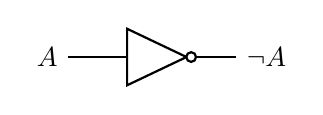
\begin{tikzpicture}[thick,circuit logic US]
\node at (0,0) (A) {$A$};
\node [not gate, anchor=input] at (1,0) (not1) {};
\draw (A) -- (not1.input);
\draw (not1.output) -- ++(0.5,0) node[right] {$\neg A$};  
\end{tikzpicture}

\end{document}
